\documentclass{article}

\usepackage{enumerate}
\usepackage{amsmath,amsthm,amssymb}
\usepackage{tikz}
\usepackage{pgfplots}
\usepackage{multicol}
%\pgfplotsset{compat=newest}

\usepackage[margin=0.5in]{geometry}

\begin{document}

\noindent \textbf{Name:}\underline{\hspace{2in}} \hfill \textbf{Handout November 1}
\\ \\

\begin{enumerate}
\item Sketch the following angles in standard position:
  \begin{multicols}{2}
    \begin{enumerate}
    \item $\theta = 13 \pi / 3$ rad \\ 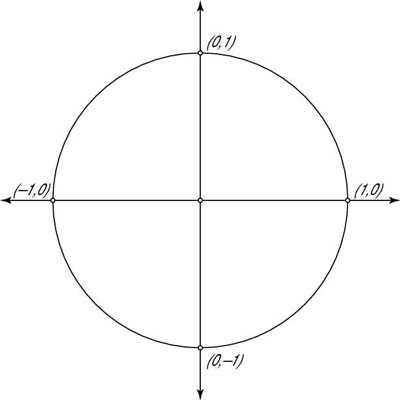
\includegraphics[scale=0.4]{circle.jpg}
    \item $\theta = -13 \pi / 3$ rad\\ 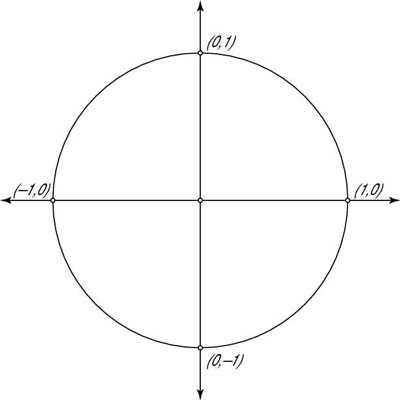
\includegraphics[scale=0.4]{circle.jpg}
    \item $\theta = 10$ rad\\ 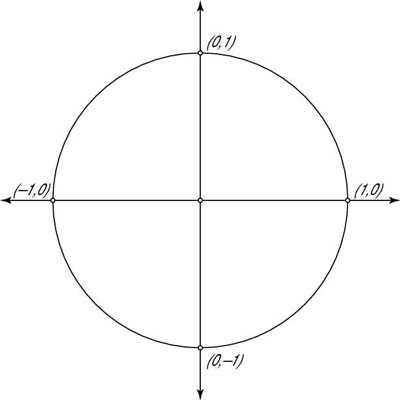
\includegraphics[scale=0.4]{circle.jpg}
    \item $\theta = -10/2 \pi$ rad\\ 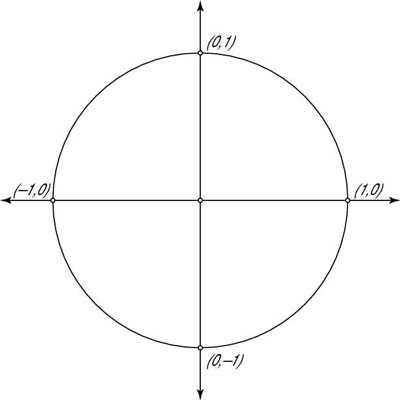
\includegraphics[scale=0.4]{circle.jpg}
    \end{enumerate}
  \end{multicols}
\item The \emph{Pythagorean Identity} is true because the point $(\cos(\theta),\sin(\theta))$ always lies on the unit circle $x^2 + y^2 = 1$. Here's the Pythagorean Identity:
  \[
    \cos^2(\theta) + \sin^2(\theta) = 1
  \]
  You should be able to write this down from memory.
  \begin{enumerate}
  \item Divide the Pythagorean Identity by $\cos^2(\theta)$ and simplify to get a new trigonometric identity.
    \vspace{1.5in}
  \item Divide the Pythagorean Identity by $\sin^2(\theta)$ and simplify to get a new trigonometric identity.
  \end{enumerate}
  \newpage
\item Given the value of one trigonometric, find the value of all the others. (Hint: Use the Pythagorean Identity and the variants you found in Question 2.)
  \begin{enumerate}
  \item 
    \begin{multicols}{2}
      $\sin(\theta) = $ \\ \\
      $\cos(\theta) = $ \\ \\
      $\tan(\theta) = $ \\ \\
      $\csc(\theta) = $ \\ \\
      $\sec(\theta) = $ \\ \\
      $\cot(\theta) = $
    \end{multicols}
    \vspace{1in}
  \item 
    \begin{multicols}{2}
      $\sin(\theta) = $ \\ \\
      $\cos(\theta) = $ \\ \\
      $\tan(\theta) = $ \\ \\
      $\csc(\theta) = $ \\ \\
      $\sec(\theta) = $ \\ \\
      $\cot(\theta) = $
    \end{multicols}
    \vspace{1in}
  \item 
    \begin{multicols}{2}
      $\sin(\theta) = $ \\ \\
      $\cos(\theta) = $ \\ \\
      $\tan(\theta) = $ \\ \\
      $\csc(\theta) = $ \\ \\
      $\sec(\theta) = $ \\ \\
      $\cot(\theta) = $
    \end{multicols}
  \end{enumerate}
  \vspace{1in}
\item Challenge Question:
\end{enumerate}

\end{document}
